\section{Construyendo aproximaciones}

\subsection{Solución Greedy}

Como es sabido el Hitting Set Problem pertenece a NP-completo y por lo tanto no existe ninguna solución que de en tiempo polinomial de una respuesta exacta en todo caso posible, pero, es posible construir una aproximación a la solución utilizando una estrategia greedy

\subsubsection{La estrategia}

Para construir una aproximación greedy se deben cumplir las siguientes reglas:

\begin{itemize}
    \item Aplicar una regla sencilla \\
    \item Debe conseguir un óptimo local al problema actual \\
    \item Se deben repetir estas reglas hasta conseguir una respuesta \\
\end{itemize}

Por lo tanto se construye la siguiente estrategia greedy para resolver el problema:

\begin{itemize}
    \item Conseguir el jugador más representativos cuya frecuencia de aparición es la más alta entre todos los jugadores \\
    \item Eliminar todos los subconjuntos en donde este jugador aparezca \\
    \item Repetir hasta que no quede ningún subconjunto de jugadores \\
\end{itemize}

\subsubsection{La implementación}

Siguiendo los pasos anteriormente mencionados se construye la implementación en python del algoritmo de aproximación greedy 

\begin{lstlisting}[language=Python, caption= aproximación greedy, label=python_code]
def aprox_hs_by_greedy(subsets: set, a: set):
    aprox_sol = set()
    missing_sets = set(range(len(subsets)))
    subsets = list(subsets)
    return _aprox_greedy(subsets, aprox_sol, missing_sets)

def _aprox_greedy(subsets: list, aprox_sol: set, missing_sets: set):
    while(not is_solution(aprox_sol, subsets)):
        diference = set()
        player = find_most_frequent_player(missing_sets, subsets)
        for i in missing_sets: 
            if has_a_player(subsets[i], player):
                diference.add(i)
        aprox_sol.add(player)
        missing_sets.difference_update(diference)
    return aprox_sol

def find_most_frequent_player(missing_sets: set, subsets: list):
    frequency = dict()
    for subset_index in missing_sets:
        for player in subsets[subset_index]:
            frequency[player] = frequency.get(player, 0) + 1
    most_frequent_player = max(frequency, key=frequency.get)
    return most_frequent_player
\end{lstlisting}

\subsubsection{Complejidad temporal}

Para analizar la complejidad temporal del algoritmo vemos que se hacen las siguientes iteraciones sobre el algoritmo: 

\begin{enumerate}
    \item Se busca al jugador más frecuente, esto es recorre $m$ subconjuntos y por cada uno de ellos sus $k$ jugadores\\
    \item Se ejecuta un ciclo while, que en el peor de los casos realiza $m$ iteraciones y en cada una de esas realiza la llamada a buscar el jugador más frecuente
\end{enumerate}

Por lo tanto se puede concluir que el algoritmo tiene la siguiente complejidad:

$$
    T(n) = O(m^2 \cdot k)
$$
Donde $k$ se puede estimar como el cardinal del mayor subconjunto perteneciente a $m$ y $m$ como el cardinal de $m$. Importante destacar que esta cota corresponde al peor caso posible y el algoritmo podría comportarse mejor de lo esperado dependiendo de la cantidad de jugadores que necesite $k$

\subsection{Solución por programación lineal}

Para construir esta aproximación se relajan las reglas implementadas en el caso de programación lineal entera y se permite que los valores de los jugadores varíen entre 0 y 1. Por lo que las ecuaciones en este caso serían:

\begin{align}
  \sum_{b_j \in B_i} b_j &\geq 1 \quad \forall B_i \in B \\
  \sum_{b_j \in B_i} b_j &\geq 1 \quad \forall B_i \in B \\
  b_j &\in [0,1] 
\end{align}
\subsubsection{Clasificación de la aproximación}

TO-DO

\subsection{Medición de las aproximaciones}
\begin{figure}[H]
    \begin{minipage}{0.5\textwidth}
        \centering
        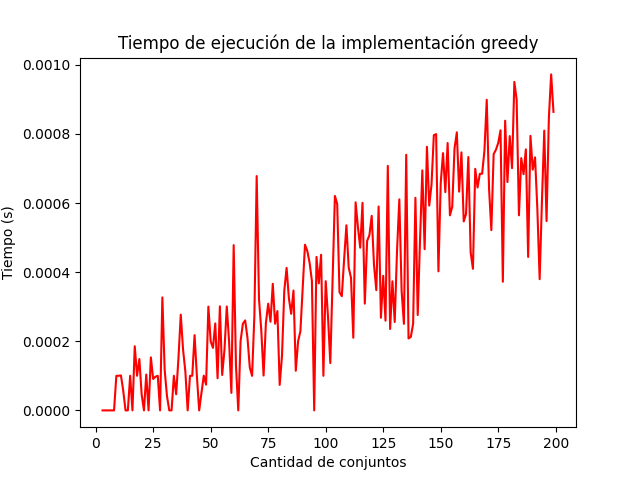
\includegraphics[width=\linewidth]{graficos/greed.png}
        \caption{Aproximación greedy}
        \label{fig:imagen1}
    \end{minipage}%
    \begin{minipage}{0.5\textwidth}
        \centering
        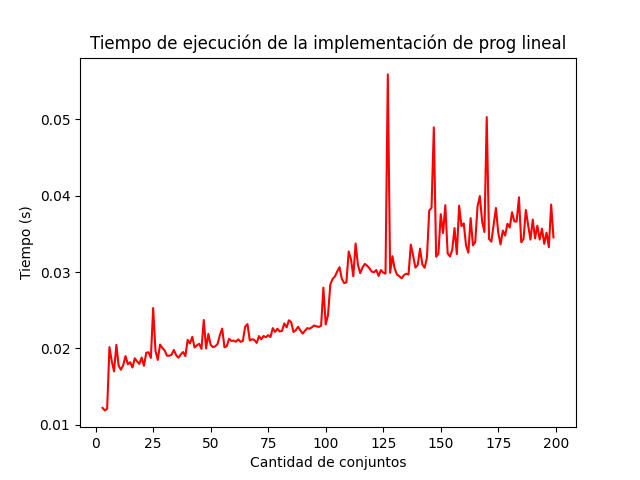
\includegraphics[width=\linewidth]{graficos/continous.png}
        \caption{Aproximación por prog. lineal}
        \label{fig:imagen2}
    \end{minipage}
\end{figure}

En las gráficas anteriores se puede observar la duración en microsegundos para el mismo set de datos utilizado a la hora de tomar mediciones sobre las soluciones exactas al problema. Se observa que la solución greedy posee una variabilidad mayor entre valores de $m$, a comparación de la solución por programación lineal que se mantiene mas estable entre los diferentes tamaños de $m$

\subsection{Comparación entre los tamaños de los óptimos}

En el siguiente gráfico se podrán observar los valores de los óptimos resultantes de ambas aproximaciones y el óptimo arrojado por una de las soluciones exactas, es fácilmente apreciable que, la aproximación por un algoritmo greedy es la cual posee el menor error a la hora de aproximar. Al mismo tiempo, se aprecia que la aproximación realizada por programación lineal no se perfila como una buena aproximación a utilizar 

\begin{figure}[H]
    \centering
    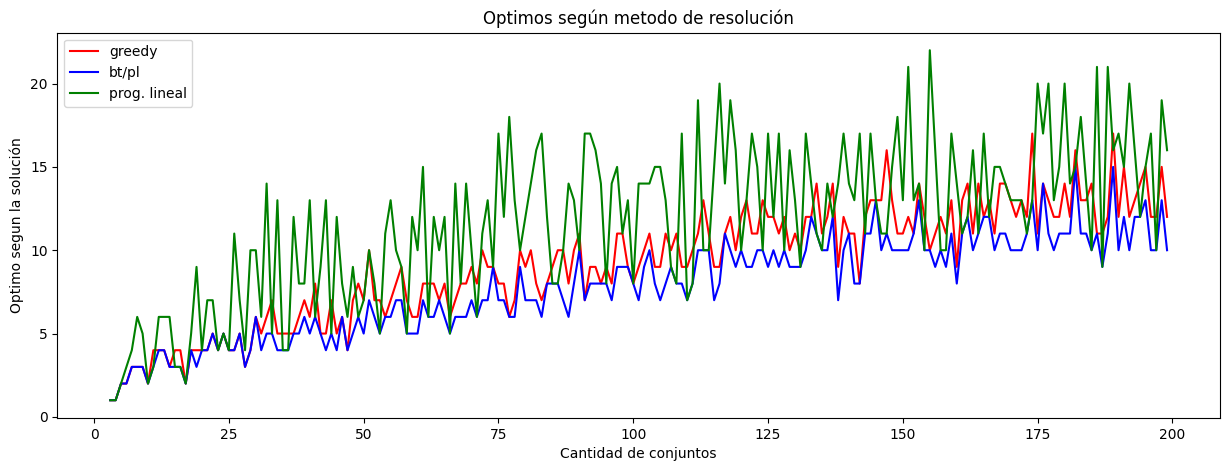
\includegraphics[width=1\textwidth]{graficos/optimos.png}
\end{figure}

En este gráfico se analizan las distancias con el óptimo real de ambas aproximaciones, confirmando una vez más que la aproximación por el algoritmo greedy tiende a distar menos del óptimo real, siendo la máxima distancia al óptimo de 5 elementos 

\begin{figure}[H]
    \centering
    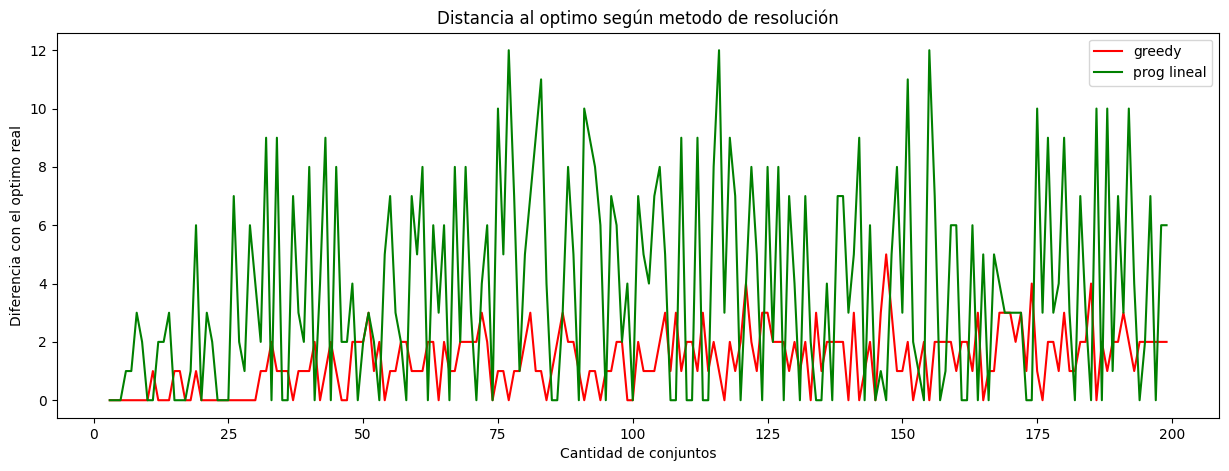
\includegraphics[width=1\textwidth]{graficos/distanciaaloptimo.png}
\end{figure}
\subsection{Mediciones en volumen de las aproximaciones}
\begin{figure}[H]
    \begin{minipage}{0.5\textwidth}
        \centering
        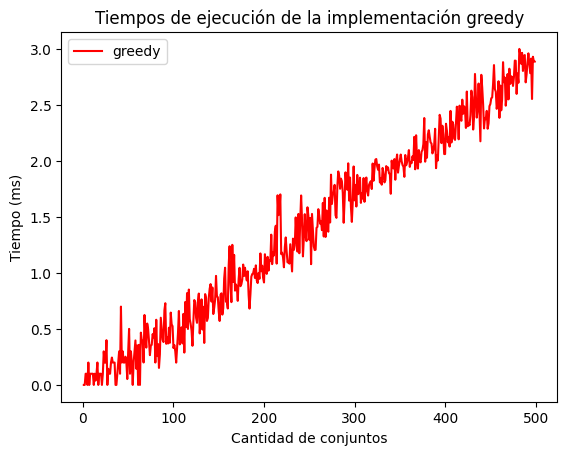
\includegraphics[width=\linewidth]{graficos/greedvol.png}
        \caption{Tiempo en vol. por greedy}
        \label{fig:imagen1}
    \end{minipage}%
    \begin{minipage}{0.5\textwidth}
        \centering
        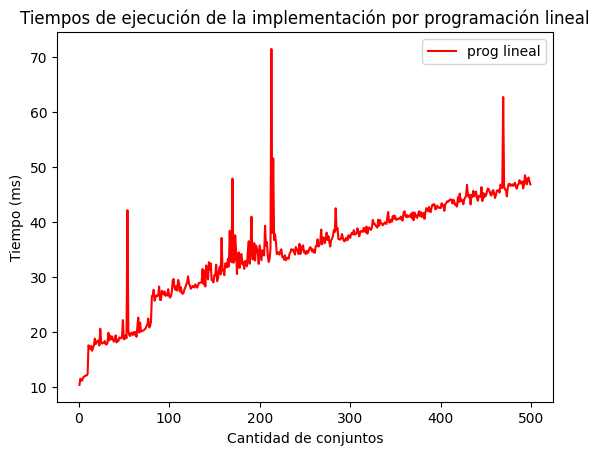
\includegraphics[width=\linewidth]{graficos/plvol.png}
        \caption{Tiempo en vol. por prog. Lineal}
        \label{fig:imagen2}
    \end{minipage}
\end{figure}
\section{Conclusión}